\documentclass[12pt]{article}
\usepackage{booktabs,ctable,multirow}
\usepackage{float}
\usepackage{array}
\usepackage{amsmath}
\usepackage{amssymb}
\usepackage{amsthm}
\usepackage{amsfonts}
\usepackage{bm}
\usepackage{soul}

\DeclareMathOperator{\C}{\mathbb{C}}
\DeclareMathOperator{\I}{\mathbb{I}}
\DeclareMathOperator{\N}{\mathbb{N}}
\DeclareMathOperator{\R}{\mathbb{R}}
\DeclareMathOperator{\Z}{\mathbb{Z}}

\DeclareRobustCommand{\E}[1]{\mathbb{E}\left[#1\right]}
\DeclareRobustCommand{\prob}[1]{\mathbb{P}\left(#1\right)}

\DeclareMathOperator{\argmax}{argmax}
\DeclareMathOperator{\argmin}{argmin}
\DeclareMathOperator{\bias}{bias}
\DeclareMathOperator{\cov}{Cov}
\DeclareMathOperator{\var}{Var}
\DeclareMathOperator{\diag}{diag}

\newcommand{\abs}[1]{\left\lvert#1\right\rvert}
\newcommand{\norm}[1]{\left\lVert#1\right\rVert}

\textheight 240mm
\textwidth  170mm
\oddsidemargin  0mm
\evensidemargin 0mm
\topmargin -20mm

\begin{document}

\begin{flushright}
    Dhamma Kimpara and Sam Zhang

    ECEN 5008-005 -- Homework \#4
\end{flushright}

\section*{Problem 1}%
\label{sec:Problem 1}

\begin{enumerate}
    \item [i)] Yes, the cost is strongly convex. Write $f_t(x) = \frac{1}{2}\norm{Ax - b_t}_2^2$, and $h_t(x) = Ax - b_t$. Then $f_t$ is $\mu$-strongly convex if the smallest eigenvalue of its Hessian $\nabla^2 f_t(x) = A$ is positive, with $\mu$ equal to that eigenvalue. By construction, then, $\mu = 1/\sqrt{\kappa}$.

    \item[ii)] We know from class that for convergence, we require the step size $\alpha$ to be in the range $(0, 2/L]$. Since $L$ is the Lipschitz constant of $\nabla f = Ax - b_t$, we have that since

        \begin{equation*}
            \norm{Ax - b_t - (Ay - b_t)} = \norm{Ax - Ay} \le \norm{A} \norm{x - y},
        \end{equation*}

        that $L \le \norm{A} = 1$, since the largest singular value of $A$ is $1$. Thus we must pick $\alpha \in (0, 2]$. The bound we derived in class uses 

        \begin{equation*}
            \rho = \max \lbrace \abs{ 1 - \alpha \mu}, \abs{ 1 - \alpha L } \rbrace = \max \lbrace \abs{ 1 - \alpha/\sqrt{\kappa}}, \abs{ 1 - \alpha } \rbrace.
        \end{equation*}

        This gives the finite bound

        \begin{equation*}
            \norm{x_t - x_t^*} \le \rho^t \norm{x_0 - x_0^*} + \sigma \sum_{i=0}^t \rho^i = \rho^t \norm{x_0 - x_0^*} + \frac{1 - \rho^{t}}{1-\rho}
        \end{equation*}

        with the asymptotic result

        \begin{equation*}
            \limsup_{t \to \infty} \norm{x_t - x_t^*} \le \frac{1}{1 - \rho}.
        \end{equation*}

        With this specific problem, since $\kappa = 100$, we have that for an arbitrary pick of $\alpha = 1$ that $rho=99/100$, so the asymptotic bound is $1/(1-\rho) = 100$. As seen in Figure \ref{fig:p1ii}, the tracking error does not appear to typically approach either the finite or asymptotic bounds here.

        \begin{figure}[h]
        \begin{center}
            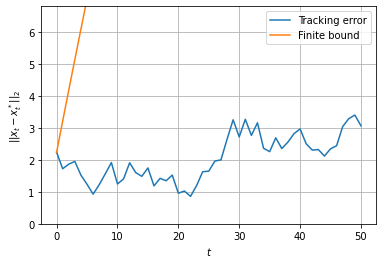
\includegraphics[scale=0.5]{figures/hw4-p1-ii.png}
        \end{center}
        \caption{Tracking error of one run of online gradient descent vs. finite bounds}
        \label{fig:p1ii}
        \end{figure}
        

\end{enumerate}



\end{document}
